\ifdefined\ishandout
\documentclass[11pt,handout]{beamer}
\else
\documentclass[11pt]{beamer}
\fi

% 日本語対応
\usepackage{luatexja}
\usepackage{luatexja-fontspec}
\renewcommand{\kanjifamilydefault}{\gtdefault}

\usepackage{mathptmx}
\renewcommand{\sfdefault}{lmss}
\renewcommand{\familydefault}{\sfdefault}
\usepackage[T1]{fontenc}
\usepackage{amsmath}
\usepackage{amssymb}
\usepackage{graphicx}
\PassOptionsToPackage{normalem}{ulem}
\usepackage{ulem}
\usepackage{caption}
\captionsetup{labelformat=empty}
\usepackage{bbm}
\usepackage{upgreek}
\setbeamertemplate{section in toc}[sections numbered]
\makeatletter
\usepackage{caption} 
\usepackage{bm}
\usepackage{subfig}
\captionsetup[table]{skip=10pt}
\newcommand\makebeamertitle{\frame{\maketitle}}%
\AtBeginDocument{%
	\let\origtableofcontents=\tableofcontents
	\def\tableofcontents{\@ifnextchar[{\origtableofcontents}{\gobbletableofcontents}}
	\def\gobbletableofcontents#1{\origtableofcontents}
}

\def\Tiny{\fontsize{7pt}{8pt}\selectfont}
\def\Normal{\fontsize{8pt}{10pt}\selectfont}

\usetheme{Madrid}
\usecolortheme{lily}
\useinnertheme{rounded}

\setbeamertemplate{footline}{\hfill\Normal{\insertframenumber/\inserttotalframenumber}}
\setbeamertemplate{navigation symbols}{}

\newenvironment{changemargin}[2]{%
	\begin{list}{}{%
			\setlength{\topsep}{0pt}%
			\setlength{\leftmargin}{#1}%
			\setlength{\rightmargin}{#2}%
			\setlength{\listparindent}{\parindent}%
			\setlength{\itemindent}{\parindent}%
			\setlength{\parsep}{\parskip}% 
		}%
		\item[]}{\end{list}}

\setbeamertemplate{footline}{\hfill\insertframenumber/\inserttotalframenumber}
\setbeamertemplate{navigation symbols}{}

\usepackage{graphicx}
\usepackage{epsfig}
\usepackage{bm}
\usepackage{epsf}
\usepackage{float}
\usepackage[final]{pdfpages}
\usepackage{multirow}
\usepackage{colortbl}
\usepackage{xkeyval}
\usepackage{listings}
\usepackage{ifthen}
\usepackage{tikz}

\usepackage{setspace}
\usepackage{ragged2e}

\setbeamersize{text margin left=1em,text margin right=1em} 

% Table formatting
\usepackage{booktabs}

% Decimal align
\usepackage{dcolumn}
\newcolumntype{d}[0]{D{.}{.}{5}}

\global\long\def\expec#1{\mathbb{E}\left[#1\right]}
\global\long\def\var#1{\mathrm{Var}\left[#1\right]}
\global\long\def\cov#1{\mathrm{Cov}\left[#1\right]}
\global\long\def\prob#1{\mathrm{Prob}\left[#1\right]}
\global\long\def\one{\mathbf{1}}
\global\long\def\diag{\operatorname{diag}}
\global\long\def\expe#1#2{\mathbb{E}_{#1}\left[#2\right]}
\DeclareMathOperator*{\plim}{\text{plim}}

\usepackage{appendixnumberbeamer}
\renewcommand{\thefootnote}{}

\setbeamertemplate{footline}
{
	\leavevmode%
\hfill
	\insertframenumber{}\hspace*{2ex}\vspace{1ex}
}

\makeatother

\usepackage[english]{babel}

\usepackage{tikz}
\newcommand*\circled[1]{\tikz[baseline=(char.base)]{             \node[circle,ball color=structure.fg, shade,   color=white,inner sep=1.2pt] (char) {\tiny #1};}} 

\makeatletter
\let\save@measuring@true\measuring@true
\def\measuring@true{%
	\save@measuring@true
	\def\beamer@sortzero##1{\beamer@ifnextcharospec{\beamer@sortzeroread{##1}}{}}%
	\def\beamer@sortzeroread##1<##2>{}%
	\def\beamer@finalnospec{}%
}
\makeatother

\setbeamersize{text margin left= .8em,text margin right=1em} 
\newenvironment{wideitemize}{\itemize\addtolength{\itemsep}{10pt}}{\enditemize}
\newenvironment{wideitemizeshort}{\itemize}{\enditemize}

\newcommand{\indep}{\perp\!\!\!\!\perp} 

\DeclareMathOperator*{\argmax}{arg\,max}
\DeclareMathOperator*{\argmin}{arg\,min}

\begin{document}
	
	%% タイトルスライド
	\begin{frame}[noframenumbering]{}
		\vspace{0.5cm}
		\title[]{第7章：操作変数法 (IV)}
		\author{Jonathan Roth}
		\date{数理計量経済学 I \\ ブラウン大学\\} 
		\titlepage {\small{}\ }\thispagestyle{empty} \vspace{-30pt}
		
	\end{frame}
	
	
	\begin{frame}{モチベーション}
		
		\begin{wideitemize}
			\item
			これまでに、観察可能な特徴を条件として、処置が実質的にランダムに割り当てられている（条件付き非交絡性）場合に、平均処置効果を推定する方法を見てきました。
			
			\item
			また、パネルデータがあり、選択バイアスが時間を通じて一定である（並行トレンド）と仮定できる場合に、条件付き非交絡性の仮定を緩和する方法も学びました。
			
			
			\pause
			
			\item
			しかし、これらの仮定が妥当ではない場合もあります。
			
			\pause
				\begin{itemize}
					{\normalsize					
					\item
					観察されない交絡変数が存在することを懸念する場合。
					
					\item
					パネルデータがない場合、あるいは交絡因子が時間とともに変化する（並行トレンドが崩れる）ことを懸念する場合。
					} 
				\end{itemize}			
			
			
			\pause
			
			\item
			そのような場合、何ができるでしょうか？ 
		\end{wideitemize}
		
	\end{frame}
	

	\begin{frame}{「局所的実験」}

		\begin{wideitemize}
			\item
			因果推論の黄金律は実験を行うことです。
			
			\item
			しかし、多くの場合、実験の実施は不可能です。
			
			\pause
			\item
			幸いなことに、関心のある処置の「受け入れ（take-up）」に影響を与えるような（自然）実験が存在することがあります。
			
			\pause
			\item
			もしそのような実験があれば、（特定の条件の下で）その実験によって処置を受けることになった人々（「コンプライヤー」）における処置の効果を学ぶことができます。
		\end{wideitemize}

	\end{frame}	

	\begin{frame}{例：Medicaid の効果}
		\begin{wideitemize}
			\item
			政策上の重要な問い：Medicaid は健康状態にどのような影響を与えるか？ 
			
			\pause
			\item
			Medicaid の因果的効果を知るための理想的な状況は、誰が加入するかをランダムに決めることです。
				\begin{wideitemize}
					\pause
					\item
					道徳的・予算的な理由から不可能です。
				\end{wideitemize}
			
			\pause
			\item
			しかし、オレゴン健康保険実験（OHIE）があります。これは、所得が連邦貧困線（FPL）の100\%から138\%の間にある人々を対象に、Medicaid の\textit{加入資格}を無作為に割り当てたものです。
		\end{wideitemize}
	\end{frame}


	\begin{frame}{復習：OHIE の背景}
		
		\includegraphics[width = 0.9\linewidth]{ohie-abstract}
	\end{frame}

	\begin{frame}{抽選の当選 vs Medicaid への加入}
		\begin{wideitemize}
			\item
			以前、OHIE を用いて「加入資格の抽選に当選すること」の因果的効果を推定しました。
			
			\item
			しかし、私たちが本当に知りたいのは「Medicaid に\textit{加入すること}」の因果的効果ではないでしょうか？ 
			
			\pause
			\item
			抽選に当選することと、Medicaid に実際に加入することは同じではありません： \medskip
			
			\begin{tabular}{lrr}
				& 当選者 (Winners) & 落選者 (Losers) \\ \hline
				Medicaid 加入経験あり & 0.397 & 0.141
			\end{tabular}
			
			\pause
			\item
			当選しても加入しない人がいます（書類を返送しなかった、加入資格を失ったなど）。
			
			\item
			落選しても、他の基準で資格を得て加入する人がいます。
		\end{wideitemize}
	\end{frame}


	\begin{frame}{Medicaid 加入がうつ病に与える影響}
		
			\begin{tabular}{lrr}
			& 当選者 & 落選者 \\ \hline
			Medicaid 加入経験あり & 0.397 & 0.141 \\
		   うつ病の症状 & 0.306 &  0.329 
		   \end{tabular}
	
	
	\begin{wideitemize}
		\item
		抽選の当選が Medicaid 加入に与える推定効果は？ \pause $0.397-0.141 = 0.256$
		
		\pause
		\item
		抽選の当選がうつ病に与える推定効果は？ \pause $0.306 - 0.329 = -0.023$
		
		\pause
		\item
		では、「Medicaid への加入」がうつ病に与える効果を推定するにはどうすればよいでしょうか？
		
		\pause
		\item
		自然な推定方法は、うつ病への効果を加入への効果で割ることです： $-0.023 / 0.256 \approx -0.09$ $\rightarrow$ 加入者1人あたり 9 ポイントの減少。
		
		\pause
		\item
		これは\textbf{操作変数法 (IV)}による推定値と呼ばれます。これはどのような場合に機能するのでしょうか？ また、どのように解釈すべきでしょうか？
	\end{wideitemize}
	
	\end{frame}


	\begin{frame}{局所平均処置効果 (LATE)}
	
	
	\begin{wideitemize}

		\item
		特定の仮定の下で、操作変数法を用いることで\textbf{局所平均処置効果} (Local Average Treatment Effect, LATE) を識別できることを示します。
		
		\pause
		\item
		これは\textbf{コンプライヤー} (compliers)、すなわち「抽選に当たったからこそ Medicaid に加入した人々」における平均処置効果です。
		
		\pause
		\item
		これが「局所的（local）」な効果であるのは、実験によって Medicaid 加入ステータスが変化しなかった人々についての効果は何も教えてくれないからです。

		\pause
		\item
		次に、操作変数法を用いて LATE を識別するために必要な仮定を確認します。
	\end{wideitemize}
		
	\end{frame}

\begin{frame}{4つのタイプの人々}

集団を以下の4つのタイプに分類できます：
	
	\begin{wideitemize}
		\item
		\textbf{オールウェイズ・テイカー} (Always-takers)：抽選の結果に関わらず、必ず Medicaid に加入する人々。
		
		\pause
		\item  \textbf{ネバー・テイカー} (Never-takers)：抽選の結果に関わらず、決して Medicaid に加入しない人々。
		
		\pause
		\item \textbf{コンプライヤー} (Compliers)：抽選に当選した場合にのみ Medicaid に加入する人々。
		
		\pause
		\item \textbf{ディファイアー} (Defiers)：抽選に落選した場合にのみ Medicaid に加入する人々。
			\begin{itemize}
				\pause
				\item 
				ディファイアーは非現実的な存在と考えられ、通常は存在しないと仮定します（\textbf{単調性}の仮定）。
			\end{itemize}
	\end{wideitemize}

\end{frame}



\begin{frame}{4つのタイプの人々 -- 数式による表現}
	
		
	\begin{wideitemize}
		\item
		$D_i$ を Medicaid に加入したかどうかの指標（処置）とします。\\
		$Z_i$ を抽選に当選したかどうかの指標（\textbf{操作変数}）とします。
		
		\pause
		\item
		潜在的結果と同様に、\textbf{潜在的処置} $D_i(1)$ と $D_i(0)$ を導入します：
			\begin{itemize}
				\item 
				$D_i(1)$： $Z_i=1$ （当選）の場合の加入ステータス。
				
				\item
				$D_i(0)$： $Z_i=0$ （落選）の場合の加入ステータス。
				
			\end{itemize}
		

		\pause
		\item
		\textbf{オールウェイズ・テイカー}： $D_i(1) = D_i(0) = 1$
		
		\pause
		\item  \textbf{ネバー・テイカー}： $D_i(1) = D_i(0) = 0$
			
		
		\pause
		\item \textbf{コンプライヤー}： $D_i(1) = 1$ かつ $D_i(0) = 0$
		
		\pause
		\item \textbf{ディファイアー}： $D_i(1) = 0$ かつ $D_i(0) = 1$
			
	\end{wideitemize}
	
\end{frame}



\begin{frame}{主要な仮定}
	\begin{wideitemize}
	\item
	\textbf{独立性} (Independence)：操作変数（例：抽選結果）は実質的にランダムに割り当てられている。 $Z_i \indep (Y_i(0),Y_i(1), D_i(0), D_i(1))$
	
	\pause
	\item
	\textbf{関連性} (Relevance)：操作変数が処置を受ける確率に影響を与える。 $P(D_i = 1 | Z_i = 1) \neq P(D_i = 1 | Z_i = 0)$
		\begin{itemize}
			\item 
			これはデータで検証可能です（実際に影響していました）。
		\end{itemize}
	
	\item
	\textbf{単調性} (Monotonicity)：ディファイアーが存在しない。すべての $i$ について $D_i(1) \geq D_i(0)$。
			\begin{itemize}
				\item 
				落選しても加入するような人が、当選したときに加入しなくなるとは考えにくいので、妥当な仮定です。
			\end{itemize}

	\end{wideitemize}	
\end{frame}


\begin{frame}{最後の重要な仮定 --- 除外制約！}
	
	\begin{wideitemize}
		\item
		最後の一つであり、しばしば最も議論の的となるのが\textbf{除外制約} (Exclusion restriction) です。
		
		\pause
		\item
		直感的には、操作変数 $Z_i$ （抽選の当選）は、\textit{処置（Medicaid 加入）を通じてのみ}アウトカムに影響を与えるという仮定です。
		
		\pause
		\item
		数学的には、 $Y_i = D_i(Z_i) Y_i(1)  + (1- D_i(Z_i)) Y_i(0) $ と書けることを意味します。
		\medskip
			\begin{itemize}
				\item 
				潜在的結果を $Y_i(d,z)$ と書くなら、 $Y_i(d,z) = Y_i(d)$ であるという仮定です。
			\end{itemize}
		
		\pause
		\item
		これは、処置ステータスが変化しないオールウェイズ・テイカーやネバー・テイカーにとっては、当選したかどうかがアウトカムに影響を与えないことを意味します。
	\end{wideitemize}
	
	
\end{frame}


\begin{frame}{なぜ除外制約が崩れるのか？}
	
\begin{wideitemize}
	\item
	操作変数（当選）が、処置ステータスを変えることなくアウトカムに直接影響を与える場合、除外制約は満たされません。
	
	\pause
	\item
	例えば OHIE において、当選したオールウェイズ・テイカーは当選しなかった場合よりも早く Medicaid に加入できたとします。これは除外制約に違反するでしょうか？
	
	\pause
	\item
	はい。Medicaid への加入「時期」が健康に直接影響を与えるのであれば、違反になります。
	 
\end{wideitemize}	
\end{frame}



\begin{frame}{図解}
	
\only<1>{\includegraphics[width=0.45\linewidth]{dags/Slide2.png}}
\only<2->{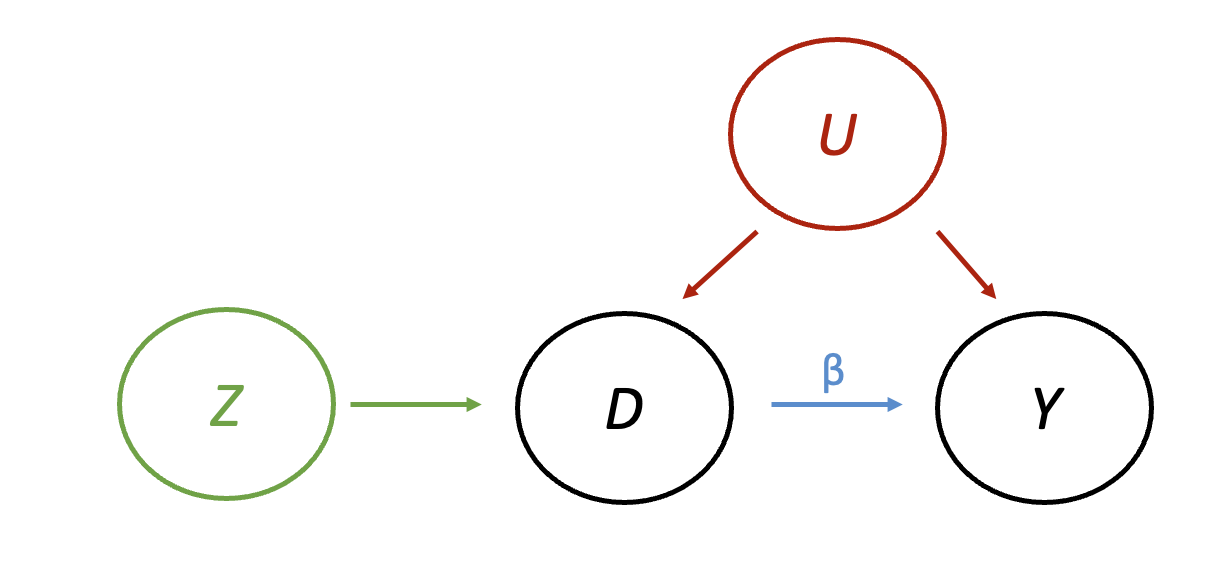
\includegraphics[width=0.45\linewidth]{dags/Slide3.png}}	
	
\begin{wideitemizeshort}
	\item
	非交絡性が満たされないのは、処置 $D$ とアウトカム $Y$ の両方に影響を与える観察されない $U$ が存在する場合です。
	
	\pause
	\item
	操作変数 $Z$ があれば、この問題を回避できます。
	
	\pause
	\item
	独立性： $Z$ は未観察因子 $U$ の影響を受けない。
	
	\pause
	\item
	除外制約： $Z$ は $D$ を通じてのみ $Y$ に影響を与える。
\end{wideitemizeshort}	
\end{frame}


\begin{frame}{LATE 定理}

	\begin{wideitemize}
		\item
		独立性、関連性、除外制約、単調性が成り立つとき：
		
		$$ \dfrac{ \color{teal} E[Y_i | Z_i = 1] - E[Y_i | Z_i = 0 ]  }{  \color{blue} E[D_i | Z_i = 1] - E[D_i | Z_i = 0 ]   }  = {\color{red} E[Y_i(1) - Y_i(0) | D_i(1) = 1, D_i(0) = 0 ] } $$
		
		\noindent 言葉で言えば：
		
		$$ \dfrac{ \color{teal} Z \text{ が } Y \text{ に与える効果}  }{  \color{blue} Z \text{ が } D \text{ に与える効果}   }  = {\color{red} \text{コンプライヤーにおける平均処置効果} } $$
		
		
		\pause
		\item
		この成果により、Joshua Angrist と Guido Imbens は 2021 年ノーベル経済学賞を受賞しました！
		
	\end{wideitemize}	
\end{frame}


\begin{frame}{LATE 定理の直感}
\begin{wideitemize}
	\item
	定理の式：
	
	$$ \dfrac{ \color{teal} E[Y_i | Z_i = 1] - E[Y_i | Z_i = 0 ]  }{  \color{blue} E[D_i | Z_i = 1] - E[D_i | Z_i = 0 ]   }  = {\color{red} \text{LATE} } $$
	
	\pause
	\item
	独立性により、{\color{teal} 分子}は $Z$ が $Y$ に与える因果的効果です。
	
	\pause
	\item
	しかし、除外制約によれば、 $Z$ の $Y$ への効果は、処置ステータスが変化しない人々（AT, NT）にとっては 0 です。 \pause また単調性によりディファイアーはいません。
	
	\pause
	\item
	したがって、{\color{teal} 分子}は「コンプライヤーにおける平均効果」に「コンプライヤーの割合」を掛けたもの、すなわち {\color{teal}  $LATE \times P(Complier)$ } になります。
	
	\pause
	\item
	一方、{\color{blue} 分母}は $Z$ が $D$ に与える効果です。これは AT や NT にとっては 0 なので、単にコンプライヤーの割合 {\color{blue}  $P(Complier)$} に等しくなります。
	
\end{wideitemize}	
\end{frame}


\begin{frame}{より形式的な導出}

\begin{wideitemize}
	\item
	集団をオールウェイズ・テイカー (AT)、ネバー・テイカー (NT)、コンプライヤー (C) の3つのグループに分けます。 \pause （ディファイアーはいないと仮定しました）。
	
	\item
	それぞれの割合を $\alpha_{AT} = P(AT), \alpha_{NT} = P(NT), \alpha_{C} = P(C)$ とします。
	
	\pause
	\item
	$Z$ はランダムに割り当てられている（独立性）ので、
	$P(AT |  Z = 1) =\pause{} P(AT) = \alpha_{AT}$ です。 \\ \pause
	同様に、 $P(AT |  Z = 0) =\pause{} P(AT) = \alpha_{AT}$ です。
	
	\pause
	\item
	同様の議論で、NT と C の割合も $Z=1$ と $Z=0$ のグループで同じになります。
\end{wideitemize}	
	
\end{frame}


\begin{frame}{より形式的な導出}

\begin{wideitemize}
	
	\item
	次のステップ：{\color{teal} 分子}が $\color{teal} \alpha_C \times LATE$ であることを示します。
	
	\pause
	
	\item 
	反復期待値の法則より：
	\begin{small}
	\begin{align*}
	 &E[Y_i | Z_i = 1]  = \pause{}\\ %
	&\alpha_C E[ Y_i | Z_i = 1, C ] +  \alpha_{AT} E[ Y_i | Z_i = 1, AT ] + \alpha_{NT}E[Y_i | Z_i  =1, NT] =\pause{}\\%
	& \alpha_C E[ Y_i(1) | Z_i = 1, C ] +  \alpha_{AT} E[ Y_i(1) | Z_i = 1, AT ] + \alpha_{NT}E[Y_i(0) | Z_i  =1, NT] = \pause{}\\
	& \alpha_C E[ Y_i(1) | C ] +  \alpha_{AT} E[ Y_i(1) | AT ] + \alpha_{NT}E[Y_i(0) |  NT]
	\end{align*} 
	\end{small}	
	\noindent 最後の行で独立性を用いました。
	\item
	同様に：
		\begin{small}
		\begin{align*}
			&E[Y_i | Z_i = 0]  = \pause{} \alpha_C E[ Y_i(0) | C ] +  \alpha_{AT} E[ Y_i(1) | AT ] + \alpha_{NT}E[Y_i(0) |  NT] %
		\end{align*} 
	\end{small}	

	\item
	したがって、比の分子は以下のようになります：
	$$ \color{teal} E[Y_i | Z_i = 1] - E[Y_i | Z_i = 0]  = \alpha_C \underbrace{(E[Y_i(1) | C]  - E[Y_i(0) | C])}_{LATE}$$  
\end{wideitemize}	
	
\end{frame}


\begin{frame}{より形式的な導出}

\begin{wideitemize}
	\item
	{\color{teal} 分子}が $\color{teal} \alpha_C \times LATE$ であることを示しました。
	
	\item
	最後に、{\color{blue} 分母}が $\color{blue} \alpha_C$ であることを示します。
	
	\pause
	\item
	分母は以下の通りです：
	
	\begin{align*}
		\color{blue} E[D_i | Z_i = 1] - E[D_i | Z_i = 0] &= \pause{}  \color{blue} Pr(AT \text{ または } C | Z_i = 1) - P(AT | Z_i = 0)  \pause{} \\
		& = \color{blue}  (\alpha_C + \alpha_{AT}) - \alpha_{AT} = \pause{}  \color{blue}  \alpha_C
	\end{align*} 


	\pause
	ゆえに： $$\dfrac{\color{teal} 分子}{ \color{blue}  分母 }	= \dfrac{\color{teal} \alpha_C \times LATE}{ \color{blue}  \alpha_C } = \color{red} LATE$$
\end{wideitemize}	
	
\end{frame}


\begin{frame}{LATE の推定}
	
	\begin{wideitemize}
		\item
		IV の仮定の下で、LATE が母平均の関数として識別されることを示しました：
		
		$$ \dfrac{ \color{teal} E[Y_i | Z_i = 1] - E[Y_i | Z_i = 0 ]  }{  \color{blue} E[D_i | Z_i = 1] - E[D_i | Z_i = 0 ]   }  = {\color{red} \text{LATE}} $$
		
		
		\item
		これをどのように推定すればよいでしょうか？
		
		\pause
		\item
		標本平均を代入すればよいのです！
		
		$$\hat\beta =  \dfrac{  \bar{Y}_{Z=1} - \bar{Y}_{Z=0}   }{ \bar{D}_{Z=1} - \bar{D}_{Z=0} } , $$
		
		\noindent ここで、例えば $\bar{Y}_{Z=1}$ は $Z_i = 1$ であるユニットの $Y_i$ の標本平均です。
		
		
		\pause
		\item
		$\hat\beta$ は IV 推定量、より正確には\textbf{二段階最小二乗法} (Two-stage Least Squares, 2SLS) 推定量と呼ばれます（その理由はすぐに明らかになります）。
	\end{wideitemize}
\end{frame}


\begin{frame}{例：Medicaid}
			\begin{tabular}{lrr}
	& 当選者 & 落選者 \\ \hline
	Medicaid 加入経験あり & 0.397 & 0.141 \\
	うつ病の症状 & 0.306 &  0.329 
\end{tabular}

\bigskip 
\begin{wideitemize}
	\item
	Medicaid の例で 2SLS 推定量を計算してみましょう。
	
	\pause
	$$ \dfrac{  \bar{Y}_{Z=1} - \bar{Y}_{Z=0}   }{ \bar{D}_{Z=1} - \bar{D}_{Z=0} }  = \pause{} \frac{0.306 - 0.329}{0.397 - 0.141}  = \pause{} -0.09$$
	
\end{wideitemize}


\end{frame}



\begin{frame}{二段階最小二乗法}

\begin{wideitemize}
	\item
	以下の2つの線形回帰を考えます：
	\begin{align}
		&Y_{i} = \gamma_0 +   Z_i \gamma_1 + \epsilon_{i} \\
		&D_i = \pi_0 + Z_i \pi_1 + u_i
	\end{align}

	\item
	OLS 推定値 $\hat\gamma_1$ と $\hat\pi_1$ は何でしょうか？
	
	\pause
	\begin{align*}
		\hat\gamma_1 = \bar{Y}_{Z=1} - \bar{Y}_{Z=0} \\ \pause{}
		\hat\pi_1 = \bar{D}_{Z=1} - \bar{D}_{Z=0}
	\end{align*}

	
	\pause
	\item
	したがって、2SLS 推定量はこれら2つの OLS 係数の比になります：
	
	$$\hat\beta =  \dfrac{  \bar{Y}_{Z=1} - \bar{Y}_{Z=0}   }{ \bar{D}_{Z=1} - \bar{D}_{Z=0} } = \frac{\hat\gamma_1}{\hat\pi_1} $$
	
	
	\pause
	\item
	式 (2) は通常「\textbf{第一段階}（first-stage）」、式 (1) は「\textbf{誘導型}（reduced-form）」と呼ばれます。
\end{wideitemize}	
	
\end{frame}


\begin{frame}{例：Medicaid}
	\begin{tabular}{lrr}
		& 当選者 & 落選者 \\ \hline
		Medicaid 加入経験あり & 0.397 & 0.141 \\
		うつ病の症状 & 0.306 &  0.329 
	\end{tabular}
	
	\bigskip 
	\begin{wideitemize}
		\item
		以下の「第一段階」回帰の係数は？
		$$D_i = \pi_0 + Z_i \pi_1 + u_i$$
		
		\pause
		\item
		$\hat\pi_1 = 0.397 - 0.141 = 0.256$
		
		\pause
		\item
		以下の「誘導型」回帰の係数は？
		$$Y_i = \gamma_0 + Z_i \gamma_1 + \epsilon_i$$
		
		\pause
		\item
		$\hat\gamma_1 = 0.306 - 0.329 = -0.023$
		
		\pause
		\item
		よって 2SLS 推定量は $\hat\gamma_1/\hat\pi_1 = -0.023/0.256 = -0.09$ となります。
	\end{wideitemize}
	
\end{frame}


\begin{frame}{コントロール変数がある場合の IV}
	\begin{wideitemize}
		\item
		しばしば、操作変数が実質的にランダムに割り当てられているという仮定は、観察可能な特徴を条件として初めて妥当になります。
		
		\item
		実際、OHIE では抽選に当たる確率は家族の人数に依存していました。
		
		\pause
		\item
		独立性の仮定を、条件付き独立性 $Z_i \indep (Y_i(1),Y_i(0),D_i(1), D_i(0)) | X_i$ に置き換えたとします。
		
		\item
		前述と同様の議論により、同じ $x$ の値を持つグループ内で同様の比をとることで、「\textbf{条件付き LATE}」を識別できます：
		
		\begin{align*}
			&\dfrac{ \color{teal} E[Y_i | Z_i = 1, X_i = x] - E[Y_i | Z_i = 0, X_i = x ]  }{  \color{blue} E[D_i | Z_i = 1, X_i = x] - E[D_i | Z_i = 0 , X_i = x]   }  = \\&{ \color{red}  \underbrace{ E[Y_i(1) - Y_i(0) | D_i(1) = 1, D_i(0) = 0, X_i = x] }_{\text{LATE(x)}} }
		\end{align*}
		
		
	\end{wideitemize}	
\end{frame}


\begin{frame}{条件付き LATE の推定}

\begin{wideitemize}
	\item
	実務において操作変数の条件付き独立性を仮定する場合、コントロール変数を含めた 2SLS の修正版を推定します。
	
	\item
	すなわち、 $\hat\beta_{2SLS} = \hat\gamma_1 / \hat\pi_1$ を用います。ここで $\hat\gamma_1, \hat\pi_1$ は以下の OLS 推定値です：
	
		\begin{align}
		&Y_{i} = \gamma_0 +   Z_i \gamma_1 + \bm{X}_i' \bm{\gamma}_2 + \epsilon_{i} \label{eqn: rf w covariates}\\
		&D_i = \pi_0 + Z_i \pi_1 + \bm{X}_i'\pi_2 +  u_i \label{eqn: fs w covariates}
	\end{align}
	
	\pause 
	
	\item
	$\bm{X}_i$ がカテゴリー変数（例：家族の人数）のダミー変数のセットである場合、これは各共変量の値における 2SLS 推定値の加重平均を与えます。
	
	\pause
	\item
	より一般的には、 (\ref{eqn: fs w covariates}) が第一段階の CEF の良い近似であれば、これは $LATE(x)$ の加重平均の近似的な一致推定量となります。
	
\end{wideitemize}

\end{frame}


\begin{frame}{例：Medicaid}
	\begin{wideitemize}
		\item
		OHIE では、抽選は家族の人数を条件としてのみランダムでした。
		
		\pause
		\item
		そのため Finkelstein et al. (2012) は、以下の 2SLS を推定しています：
		
			\begin{align}
			&Y_{i} = \gamma_0 +   Z_i \gamma_1 + \bm{X}_i' \bm{\gamma}_2 + \epsilon_{i} \\
			&D_i = \pi_0 + Z_i \pi_1 + \bm{X}_i'\pi_2 +  u_i 
		\end{align}
		
		\noindent ここで $\bm{X}_i$ には家族の人数の固定効果やその他の人口統計学的変数が含まれています。
					
	\end{wideitemize}
\end{frame}


\begin{frame}
	\centering
	\includegraphics[width = 0.9\linewidth]{finkelstein-results-er}
\end{frame}


\begin{frame}
	\centering
	\includegraphics[width = 0.9\linewidth]{finkelstein-results-depression}
\end{frame}


\begin{frame}{「擬似実験」的な操作変数}
	
	\begin{wideitemize}
		\item
		Medicaid の事例では、操作変数 $Z_i$ は明示的にランダムに割り当てられていました。
		
		\pause
		\item
		他の設定では、直接ランダム化されたわけではないが、潜在的に「ランダムと同様」と見なせるような特異な要因による操作変数を用いることがあります。
		
		\item
		これにより IV を利用できるケースが広がりますが、必要な仮定についてはより厳格な吟味が必要になります！
	\end{wideitemize}
\end{frame}


\begin{frame}{例：Angrist and Krueger (1991)}
	\begin{wideitemize}
		\item
		AK (1991) は労働経済学の古典的な問いに取り組んでいます：教育を1年追加することの労働市場における収益（賃金への影響）は何か？ 
		
		\pause
		\item
		単に教育年数が長い人と短い人の賃金を比較するだけではいけないのはなぜでしょうか？
			\pause
			\begin{itemize}
				\item 
				教育年数はランダムに決まるわけではないからです。教育の選択は、能力や家庭環境などの、賃金に直接影響を与える多くの交絡因子に依存している可能性があります。
			\end{itemize}
		
		\pause
		\item
		IV を用いて教育の収益を推定するには何が必要でしょうか？
		
		\pause
		\item
		実質的にランダムに割り当てられ、教育年数を通じてのみ賃金に影響を与えるような操作変数を見つける必要があります。
	\end{wideitemize}
\end{frame}


\begin{frame}{義務教育法}
	\begin{wideitemize}
		\item
		米国のほとんどの州には、16歳または17歳の誕生日まで学校に留まることを義務付ける義務教育法があります。
		
		\pause
		\item
		AK は、これらの法律により、中退を考えている生徒は、1年のうちの早い時期に生まれた場合、より少ない教育しか受けられなくなると主張しました。
		
		\item
		つまり、同じ学年で最も年上の子（1月1日生まれ）と最も若い子（12月31日生まれ）を比べると、年上の子は最も若い子よりも1年早く合法的に中退できてしまいます。
		
		
		\pause
		\item
		AK は、1年のうちのどの時期に生まれるかは実質的にランダムであると議論し、教育年数の操作変数として「出生四半期」を用いました。
	\end{wideitemize}
\end{frame}


\begin{frame}{}
	\centering
	\includegraphics[width = 0.7 \linewidth]{ak-first-stage-graph}
	
	\begin{wideitemize}
		\item
		実際に AK は、第1四半期に生まれた人は、同じ年のそれ以外の四半期に生まれた人よりも平均して教育年数が短いことを見出しました。
	\end{wideitemize}
\end{frame}

\begin{frame}
	\centering
	\includegraphics[width = 0.7 \linewidth]{ak-first-stage-basic}
	
	\pause
	\begin{wideitemize}
		\item
		第一段階の推定値は？ \pause{} $11.5252 - 11.3996 = 0.1256$
		
		\pause
		\item
		誘導型の推定値は？ \pause{} $5.1574 - 5.1484 = 0.0090$
		
		\pause
		\item
		2SLS 推定値は？ \pause{} $0.0090 / 0.1256 = 0.0715$
	\end{wideitemize}
\end{frame}


\begin{frame}
	\centering
	\includegraphics[width = 0.9 \linewidth]{ak-first-stage}
\end{frame}


\begin{frame}{仮定の評価}
	\begin{wideitemize}
		
		\item \textbf{関連性：} \pause 出生四半期が教育年数と相関している必要がある。 \pause{} \\
		$\checkmark$ これは検証可能であり、実際に相関していました（$t$ 統計量は 12）。
		
		
		\pause
		\item \textbf{独立性：} \pause 出生四半期が、賃金の決定要因や義務教育法への反応と独立である必要がある（ $Z_i \indep (Y(.), D(.))$ ）。 
		
		\pause
		\item
		親が子供の誕生時期を正確にコントロールできないのであれば、独立性は妥当に見えます。 \pause しかし...
	\end{wideitemize}	
	
\end{frame}

\begin{frame}
\centering
\includegraphics[width = 0.8\linewidth]{qob-characteristics}

\begin{wideitemize}
	\item
	出生四半期は、いくつかの人口統計学的特徴と相関しています。
	
	\item
	これは独立性の仮定が満たされていない可能性を示唆しています。
\end{wideitemize}
\end{frame}


\begin{frame}{仮定の評価...}
	
	\begin{wideitemize}
		\item
		\textbf{除外制約：} 出生四半期は教育年数を通じてのみ賃金に影響を与える。
		
		\pause
		\item
		これは、出生四半期によって教育年数が変化しない人々にとっては、いつ生まれても賃金が同じであることを意味します。
		
		\pause
		\item 
		一般的は妥当そうですが... \pause 学年の中で相対的に年上か年下かということが、教育の質に直接影響を与えるかもしれません。
					
	\end{wideitemize}
\end{frame}


\begin{frame}
	\centering
	\includegraphics[width = 0.7\linewidth]{nhl-births}
\end{frame}

\begin{frame}
	\centering
	\includegraphics[width = 0.7 \linewidth]{qob-disabilities}
\end{frame}

\begin{frame}{仮定の評価}
	\begin{wideitemize}
		\item
		\textbf{単調性：} 第1四半期に生まれなかった方が、全員が少なくとも同等以上の教育年数を得る。
		
		\pause
		\item
		すべての学校が1月1日を学年の区切りにしていれば妥当です。
		
		\pause
		\item
		もし9月1日を区切りにしている学校があれば、第4四半期生まれの方が教育年数が短くなる可能性もあります。
	\end{wideitemize}
\end{frame}


\begin{frame}
	\centering
	\includegraphics[width = 0.7 \linewidth]{qob-placebo}
	
	\bigskip
	
	\pause
	\begin{wideitemize}
		\item
		義務教育法（CSL）の対象年齢が異なる州を比較したところ、出生四半期の教育への影響は CSL を通じて生じていることが示唆されました。これは独立性に関する懸念をいくらか和らげるものです。
	\end{wideitemize}
\end{frame}

\begin{frame}{誰に対する処置効果か？}
	\begin{wideitemize}
		\item
		IV の仮定が（近似的に）成り立つとしましょう。
		
		\item
		推定された効果をどう解釈すべきでしょうか？ 
		
		\pause
		\item
		それはコンプライヤーに対する局所平均処置効果 (LATE) です。この場合は、「1年の後半に生まれていれば、もう1年長く学校に通ったであろう人々」に対する効果です。
		
		\pause
		\item
		なぜ LATE が全集団の ATE と一致しない可能性があるのでしょうか？
		
			\pause
			\begin{wideitemize}
				\item
				中退するかどうかの境界線上にいる人々にとっての教育の収益は、他の人々とは異なる可能性があるからです。
			\end{wideitemize}
	\end{wideitemize}
	
\end{frame}


\begin{frame}{複数の操作変数}
	\begin{wideitemize}
		\item
		これまでは、2値の操作変数（当選 vs 落選）を考えてきました。
		
		\item
		しかし、操作変数が多値をとる場合や、複数の異なる操作変数がある場合もあります。
		
		
		\item
		次に、多値の操作変数からの変動をどのように利用できるかを議論します。
				
	\end{wideitemize}
\end{frame}

\begin{frame}{例：Angrist (1990)}
	\begin{wideitemize}
		\item
		Angrist (1990) は以下の問いに興味を持っています：軍隊に従事すること（特にベトナム戦争）は、その後の人生の労働賃金にどのような影響を与えるか？ 
		
		\pause
		\item
		なぜ単に退役軍人と非退役軍人を比較するだけではいけないのでしょうか？
			\pause
			\begin{itemize}
				\item 
				退役軍人ステータスはランダムではないからです。彼らはキャリアの目標、家庭環境、身体能力などの面で異なっている可能性があります。
			\end{itemize}
		
		\pause
		\item
		IV を使うには何が必要でしょうか？ \pause 実質的にランダムで、軍への入隊を通じてのみ賃金に影響を与える操作変数です。
	\end{wideitemize}
\end{frame}

\begin{frame}{Angrist (1990) -- 徴兵抽選}
	\begin{wideitemize}
		\item
		Angrist (1990) は、ベトナム戦争中に（男性を対象とした）強制的な徴兵制があったことを利用しました。
		
		\item
		1970年代、軍は抽選を行い、各誕生日にランダムに優先番号を割り当てました。番号が小さい日に生まれた人から順に徴兵の対象となりました。
		
		\pause
		\item
		抽選番号は、入隊するかどうかを完全には決定しませんでした：
		
			\begin{itemize}
				\item 
				番号が小さくても、医学的な免除を受けたり、国外へ逃れたりする人がいました。
				
				\item
				番号が大きくても、自ら志願して入隊する人がいました。
			\end{itemize} 
		
		\pause
		\item
		Angrist はまず操作変数を2値化（徴兵対象の誕生日 vs 対象外）して考え、次に多値の操作変数（各誕生日ごとの変数）へと一般化しました。
	\end{wideitemize}
\end{frame}


\begin{frame}{IV 仮定の評価}
	\begin{wideitemize}
		\item
		\textbf{独立性：} \pause 抽選番号が、潜在的な賃金や入隊傾向と系統的に関連していないこと。 \pause
			\begin{itemize}
				\item 
				抽選のランダム化により、この仮定は非常に妥当です。
				\item
				番号の大小で、観察可能な特徴に差はありません。
			\end{itemize}
		
		\item
		\textbf{除外制約：} \pause 抽選番号が入隊を通じてのみ賃金に影響を与えること。
			\pause
			\begin{itemize}
				\item 
				この文脈での除外制約は少し巧妙です。
				
				\item
				ネバー・テイカーは、番号が小さいと（徴兵を避けるために）国外へ逃げなければならなかったかもしれません。
				
				\item
				オールウェイズ・テイカーは、自ら志願した場合と徴兵された場合で、軍での経験が異なるかもしれません。
			\end{itemize}
		
		
		\item
		\textbf{関連性：} \pause 抽選番号が入隊に影響を与えること。 \pause 
			\begin{itemize}
				\item 
				妥当であり、実際に影響していました。
			\end{itemize}
		
		\pause
		\item
		\textbf{単調性：} 番号が大きくても入隊する人は、番号が小さければ必ず入隊する。 \pause
			\begin{itemize}
				\item 妥当と思われます。
			\end{itemize}
		
	\end{wideitemize}
\end{frame}


\begin{frame}
	\begin{wideitemize}
		\item
		Angrist はまず、誕生日を徴兵対象（eligible）と対象外（non-eligible）にグループ分けした2値版の操作変数を考えました。
		
		\item
		以下はその第一段階の結果です（ $\hat{p}^e - \hat{p}^n$ を参照）。
	\end{wideitemize}
\centering
\includegraphics[width = 0.7 \linewidth]{angrist-first-stage}
\end{frame}


\begin{frame}
	\centering
	\includegraphics[width = 0.9 \linewidth]{angrist-wald}
\end{frame}


\begin{frame}{この例における LATE の可視化}
	
	図解は \href{https://www.dropbox.com/s/nddh9vb6pjxvlng/2sls\%20diagrams.pdf?dl=0}{\underline{こちら}} を参照してください。
\end{frame}

%
%{	\begin{landscape}
%	\setbeamercolor{background canvas}{bg=}
%	\includepdf{2sls diagrams.pdf}
%	\end{landscape}
%
%}




\begin{frame}
	\centering
	\includegraphics[width =0.9 \linewidth]{angrist-plot}
\end{frame}

\begin{frame}{複数の操作変数を用いた 2SLS の定式化}
	\begin{wideitemize}
		\item
		この手続きは、複数の操作変数を用いた二段階最小二乗法として定式化できます。
		
		\item
		操作変数のベクトル $\bm{Z}_i$ があるとします（例： $Z_1$ は誕生日1、 $Z_2$ は誕生日2、...）。

\end{wideitemize}
\end{frame}

\begin{frame}{複数の操作変数を用いた 2SLS}
\begin{wideitemize}
		\item
		ステップ 1（第一段階）：OLS 回帰により $E[D_i | \bm{Z}_i]$ を推定する：
		
		$$D_i = \gamma_0 + \bm{Z}_i' \bm{\gamma}_1 + u _i$$
		
		（例：各誕生日ごとの平均入隊率を推定する）
		\pause
		\item
		ステップ 2：各ユニット $i$ について $E[D_i | \bm{Z}_i]$ の予測値を構築する：
		
		$$\hat{D}_i = \hat\gamma_0 + \bm{Z_i}' \bm{\hat\gamma}_1$$
		
		（例： $\hat{D}_i$ はユニット $i$ と同じ誕生日の人の平均入隊率）
		
		\pause
		\item
		ステップ 3（第二段階）： $Y_i$ を $\hat{D}_i$ に OLS 回帰する：
		
		$$Y_i = \beta_0 + \hat{D}_i \beta_1 + \epsilon_{i}$$
		
		（例：賃金を誕生日ごとの平均入隊率に回帰する）
		
		
		\pause
		\item
		$\hat\beta_1$ が（加重）LATE の推定値となります。
	\end{wideitemize}


\end{frame}


\begin{frame}
	\centering
	\includegraphics[width = 0.9 \linewidth]{angrist-2sls}
\end{frame}


\begin{frame}{Martin and Yurukoglu (2017)}
	
	\begin{wideitemize}
		\item
		Martin and Yurukoglu は以下の問いに興味を持っています：Fox News（保守的なテレビ局）への露出は、米国の投票行動にどのように影響するか？ 
		
		\item
		Fox News をよく見る地域とそうでない地域の投票行動を比較するだけで、因果的効果が得られるでしょうか？ \pause
		 	\begin{itemize}
		 		\item 
		 		おそらく得られません！ 政治的傾向という強力な交絡因子があるからです（保守的な人ほど Fox News を見、かつ共和党に投票する）。
		 	\end{itemize}
	 	
	 	\item
	 	実質的にランダムで、視聴数を通じてのみ投票に影響する操作変数が必要です。何かアイデアはありますか？ \pause
	 	
	 	\item
	 	彼らは、ケーブルテレビの「チャンネル・ラインナップにおける位置」を IV として使うことを提案しました。
	 		\begin{itemize}
	 			\item 
	 			番組ガイドの早い位置にあるほど、Fox News はよく見られる傾向があります。
	 			\item
	 			ラインナップの位置は、1990年代のケーブルニュース導入時の特異な要因によって決まっており、ランダムと同様であると議論しました。
	 		\end{itemize}
	\end{wideitemize}
\end{frame}


\begin{frame}{Martin and Yurukoglu の 2SLS 仕様}
	第一段階： 
	$$D_{i} = \pi Z_i + \boldsymbol{\gamma}' \boldsymbol{X}_i + u_i $$
	ここで $D_{i}$ は郵便番号 $i$ における1週間あたりの Fox News 平均視聴時間、 $\boldsymbol{X}_i$ は州・郡の固定効果、MSNBC の位置、人口統計学的変数（所得、年齢、人種など）を含むコントロール変数のベクトルです。 \medskip
	
	第二段階：
	$$Y_{i} = \beta \hat{D}_i + \boldsymbol{\delta}' \boldsymbol{X}_i + \epsilon_i $$
	
	\noindent ここで $Y_{i}$ は2008年選挙における共和党得票率、 $\hat{D}_i$ は第一段階からの予測値です。
\end{frame}

\begin{frame}{仮定の評価}
	\begin{wideitemize}
		\item
		\textbf{独立性：} \pause Fox News の位置が（観察可能な特徴を条件として）実質的にランダムであること。 \pause これが最も議論の余地があります。需要の高い場所ほど Fox News を早い位置に置くのではないか、という懸念があります。
		
		\item
		\textbf{除外制約：} \pause チャンネルの位置が視聴数を通じてのみ投票に影響すること。 \pause 比較的妥当に見えます。
		
		\item
		\textbf{関連性：} \pause 位置が視聴数に影響すること。 \pause 実際に影響していました。
		
		\item
		\textbf{単調性：} \pause 位置が早くなるほど、視聴数が増える（または減らない）こと。 \pause 概ね妥当ですが、遅い位置の方が他の人気チャンネルに近くて視聴が増える、といったことがあれば違反になります。
	\end{wideitemize}
\end{frame}

\begin{frame}{第一段階}
		\centering
		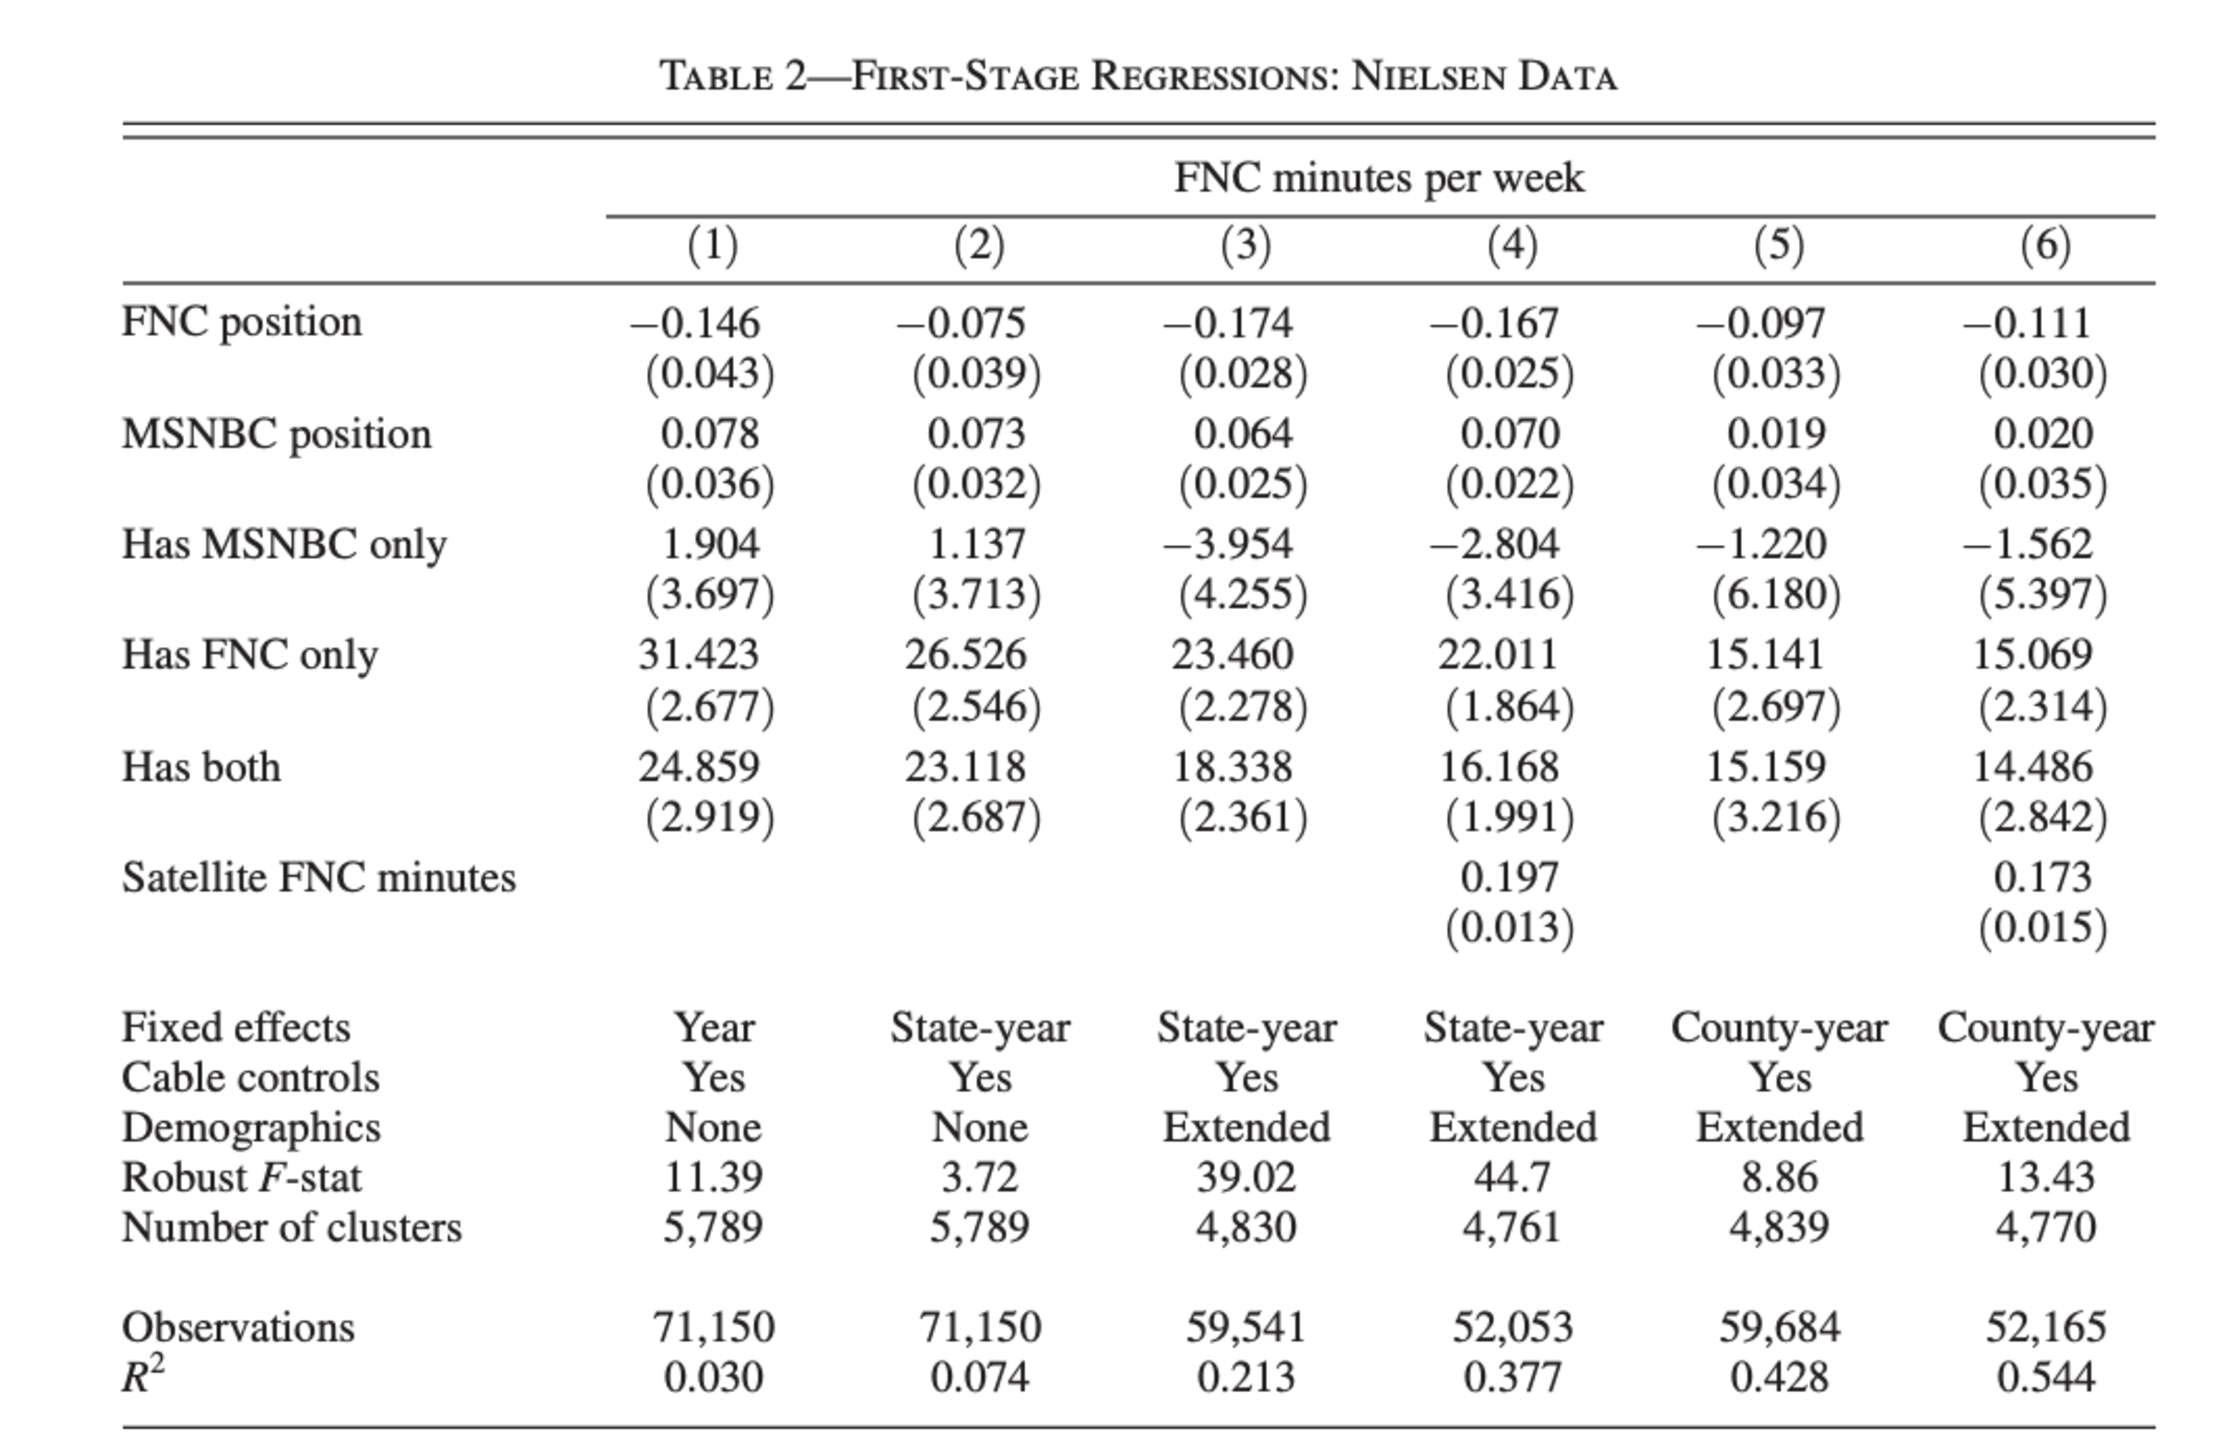
\includegraphics[width = 0.8 \linewidth]{my-first-stage}
		
		\begin{wideitemizeshort}
			\item
			ラインナップの後ろの方にあるほど、視聴数が少なくなっています。ラインナップ位置が 1 標準偏差改善すると、視聴数は週に約 2.5 分増加します。
		\end{wideitemizeshort}
\end{frame}

\begin{frame}{独立性に関する証拠}
	
 	\centering
 	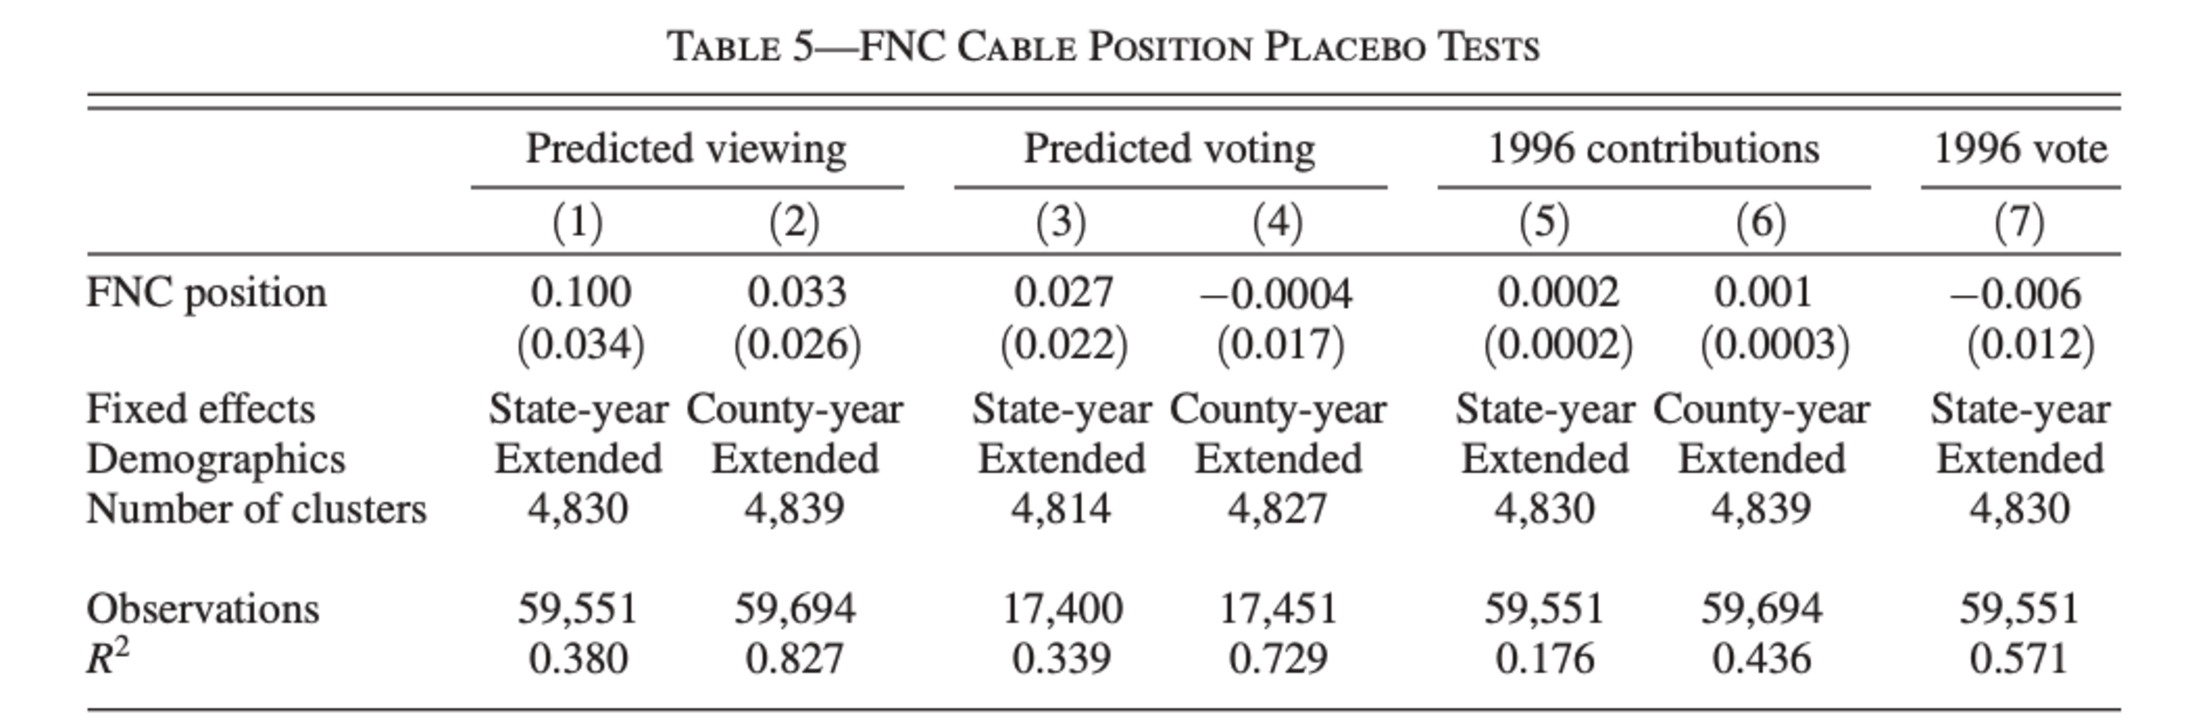
\includegraphics[width = 0.8 \linewidth]{my-balance}
	\begin{wideitemize}
		\item
		Fox News の位置は、1996年（ケーブルニュース普及前）の得票率や、ほとんどの人口統計学的特徴と有意な関連がありません。
	\end{wideitemize}
\end{frame}

\begin{frame}{衛星放送視聴者を用いた検証}
		\centering
		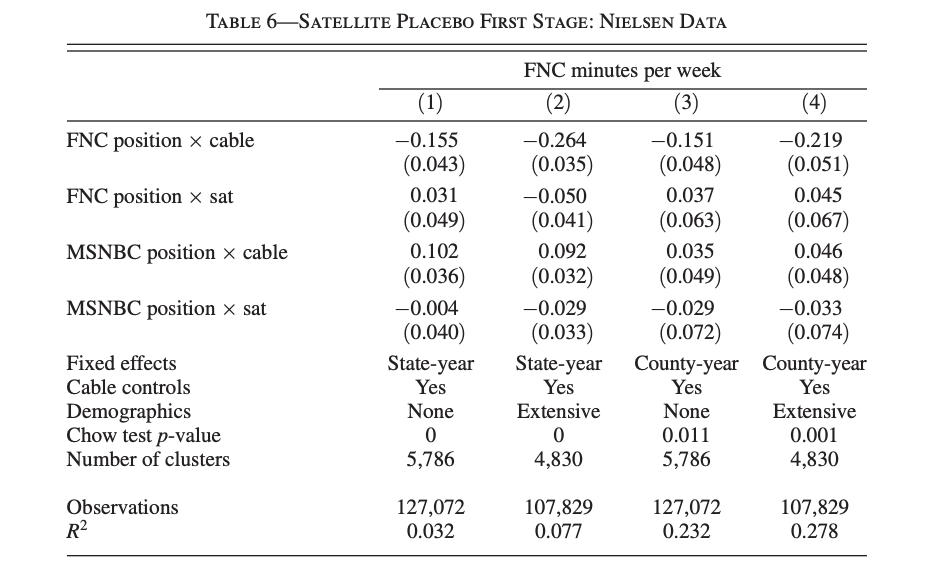
\includegraphics[width=0.7\linewidth]{my-satellite}
		\begin{wideitemize}
			\item
			チャンネル位置が視聴数を予測するのは（そのラインナップを使っている）ケーブルテレビ利用者のみであり、別のラインナップを使っている衛星放送利用者には影響していません。
		\end{wideitemize}
\end{frame}


\begin{frame}{2SLS の結果}
	\begin{center}
		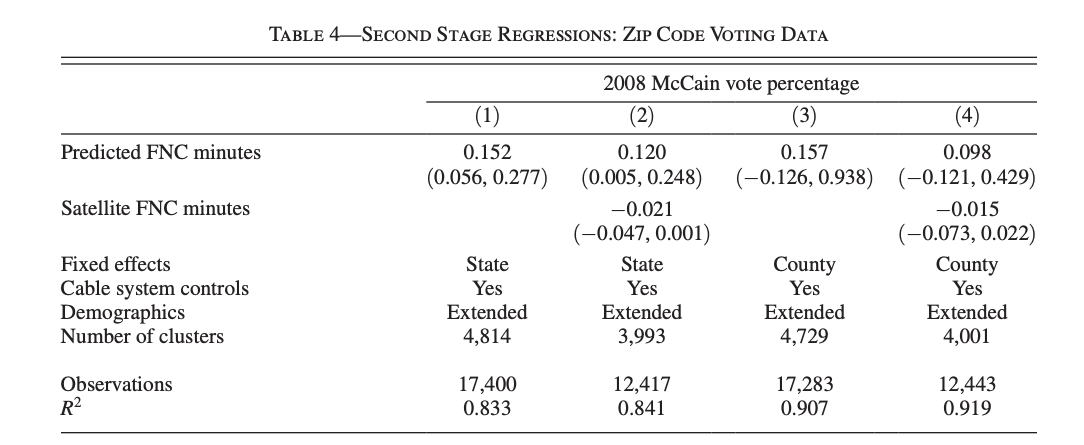
\includegraphics[width=0.9\linewidth]{my-iv}
	\end{center}
	
	チャンネル位置の 1 標準偏差の改善は視聴数を週 2.5 分増加させ、それにより共和党得票率が 0.3 ポイント上昇したと推定されました。
\end{frame}

\begin{frame}{2SLS の推論}
	\begin{wideitemize}
		\item
		2SLS 推定値の標準誤差をどのように求めればよいでしょうか？
		
		\pause
		\item
		2SLS は、第一段階の予測値 $\hat{D}$ を説明変数として OLS を実行するのと同等であることを見ました。
		
		\pause
		\item
		しかし、単にその第二段階の OLS を実行して、その OLS 標準誤差をそのまま使うのは間違いです。 \pause $\hat{D}$ 自体が推定値である（誤差を含んでいる）ことを考慮に入れていないからです。
		
		\pause
		\item
		幸い、Stata などのソフトウェアを使えば、正しい 2SLS 標準誤差を簡単に得ることができます。
			\begin{itemize}
				\item
				Stata では \texttt{ivregress 2sls y x (d=z), r} と入力します。
			\end{itemize}
		
		\pause
		\item
		これらの標準誤差はどこから来ているのでしょうか？ 
	\end{wideitemize}
\end{frame}


\begin{frame}{第一段階と誘導型の正規性}
	\begin{wideitemize}
		\item
		単一の操作変数の場合、 $\hat\beta_{IV} = \hat\gamma_1 / \hat\pi_1$ でした。ここで $\hat\gamma_1, \hat\pi_1$ は以下の OLS 推定値です：
		\begin{align*}
			&Y_{i} = \gamma_0 +   Z_i \gamma_1 + \epsilon_{i} \\
			&D_i = \pi_0 + Z_i \pi_1 + u_i
		\end{align*}
	
		\pause
		\item
		OLS 推定値が漸近的に正規分布に従うことは既に示しました（これらは同時にも成立します）：
		
		$$\sqrt{N}\left( \left( \begin{array}{ll} \hat\gamma_1 \\ \hat\pi_1 \end{array} \right)- \left( \begin{array}{ll} \gamma_1 \\ \pi_1 \end{array} \right) \right) \rightarrow_d \mathrm{N}(0,\Sigma)$$
	
		\pause
		\item
		これを用いて $\hat\gamma_1 / \hat\pi_1$ の漸近分布を導けるでしょうか？
	\end{wideitemize}
\end{frame}

\begin{frame}{デルタ法}
	\begin{wideitemize}
	\item
	$g(\hat\gamma_1, \hat\pi_1) = \hat\gamma_1 / \hat\pi_1$ とします。 \pause $(\hat\gamma_1, \hat\pi_1) \approx (\gamma_1, \pi_1)$ のとき、一次のテイラー展開により：
	$$g(\hat\gamma_1, \hat\pi_1) \approx g(\gamma_1,\pi_1) + \nabla g(\gamma_1,\pi_1) (\hat\gamma_1 - \gamma_1, \hat\pi_1 - \pi_1)' $$
	
	\noindent ここで $\nabla g(\gamma_1,\pi_1)$ は $(\gamma_1, \pi_1)$ における $g$ の勾配（ベクトル）です。
	
	\item
	これは次を意味します：
	
	$$\sqrt{N}\left( \underbrace{ \frac{\hat\gamma_1}{\hat\pi_1}}_{g(\hat\gamma_1 , \hat\pi_1)} -  \underbrace{\frac{\gamma_1}{\pi_1} }_{g(\gamma_1,\pi_1)} \right) \approx  \nabla g(\gamma_1, \pi_1)\sqrt{N}\left( \left( \begin{array}{ll} \hat\gamma_1 \\ \hat\pi_1 \end{array} \right)- \left( \begin{array}{ll} \gamma_1 \\ \pi_1 \end{array} \right) \right)  $$
	
	\pause
	\item
	連続写像定理より、これは $\mathrm{N}(0,  \nabla g(\gamma_1, \pi_1) \Sigma  \nabla g(\gamma_1, \pi_1)')$ に分布収束します。
	
	\pause
	\item
	分散は標本対応物（例： $\nabla g(\hat\gamma_1, \hat\pi_1)$）を用いて推定できます。
\end{wideitemize}
\end{frame}

\begin{frame}{弱識別 (Weak Identification)}
	\begin{wideitemize}
		\item
		注意： $\hat\beta_{IV} = \hat\gamma_1 / \hat\pi_1$ が定義されるのは $\hat\pi_1 \neq 0$ のときのみです。
		
		\item
		$\hat\pi_1 \rightarrow 0$ となると、 $|\hat\beta_{IV}| \rightarrow \infty$ となり、 $\hat\pi_1 \approx 0$ のとき IV 推定量の挙動は非常に不安定になります。
		
		\pause
		\item
		これまでの漸近理論では、 $\pi_1 \neq 0$ （関連性）を仮定し、 $N$ が大きくなれば $\hat\pi_1 \rightarrow_p \pi_1$ となるため、 $\hat\pi_1$ が 0 に近くなる確率は 0 に収束し、問題になりませんでした。
		
		\pause
		\item
		しかし実務上、 $\hat\pi_1$ が（標準誤差に対して）非常に 0 に近い場合があります。
		
		\item
		この場合、上記の正規分布による近似は、 $\hat\beta_{IV}$ の分布を適切に捉えることができません。これは「\textbf{弱識別}」問題として知られています。
	\end{wideitemize}
\end{frame}


\begin{frame}{弱操作変数 -- モンテカルロ・シミュレーション}
モンテカルロ・シミュレーション：真の処置効果は 0\\
$Y_i(d)= \eta + \nu; \hspace{1cm}  D_i = \pi_1 Z_i + \eta; \hspace{1cm}  \eta, \nu, Z_i \sim N(0,1)$ 	\\

\pause{}
ケース1：強い第一段階 ($\pi_1 =1$) $\rightarrow$ $\pi_1 / SD(\pi_1) \approx 22$

\centering
\includegraphics[width = 0.45 \linewidth]{fs-strong} \pause{} \includegraphics[width = 0.45 \linewidth]{iv-strong}
\end{frame}


\begin{frame}{弱操作変数 -- モンテカルロ・シミュレーション}
	モンテカルロ・シミュレーション：真の処置効果は 0\\
	$Y_i(d)= \eta + \nu; \hspace{1cm}  D_i = \pi_1 Z_i + \eta; \hspace{1cm}  \eta, \nu, Z_i \sim N(0,1)$ 	\\
	
	ケース2：中程度の第一段階 ($\pi_1 =0.25$) $\rightarrow$ $\pi_1 / SD(\pi_1) \approx 7$
	
	\centering
	\includegraphics[width = 0.45 \linewidth]{fs-medium} \pause{} \includegraphics[width = 0.45 \linewidth]{iv-medium}
\end{frame}


\begin{frame}{弱操作変数 -- モンテカルロ・シミュレーション}
	モンテカルロ・シミュレーション：真の処置効果は 0\\
	$Y_i(d)= \eta + \nu; \hspace{1cm}  D_i = \pi_1 Z_i + \eta; \hspace{1cm}  \eta, \nu, Z_i \sim N(0,1)$ 	\\
	
	ケース3：非常に弱い第一段階 ($\pi_1 =0.01$) $\rightarrow$ $\pi_1 / SD(\pi_1) \approx 0.3$
	
	\centering
	\includegraphics[width = 0.45 \linewidth]{fs-weak} \pause{} \includegraphics[width = 0.45 \linewidth]{iv-weak}
\end{frame}

\begin{frame}{複数の操作変数がある場合の弱 IV}
	\vspace{0.2cm}
	多くの操作変数がある場合にも、概念的に関連した問題が生じます。 \pause{}
	
	\begin{itemize}
		\item 典型的な例：Angrist and Krueger (1991) は、出生四半期と「出生年・州」の交差項を操作変数として用いました。 \pause{}
		\vspace{0.1cm}
		\item これにより標本内の $D_i$ の予測精度は上がりますが、標準誤差は減少します。 \pause{}
		\vspace{0.1cm}
		\item しかし Bound et al. (1995) は、ランダムに生成した操作変数を使っても、彼らと同じ 2SLS 推定値が得られてしまうことを示しました。
	\end{itemize}
	\pause{}
	\vspace{0.4cm}
	
	直感：第一段階で多くの操作変数を使うと、 $D_i$ を「過学習（overfit）」してしまいます。 \pause{}
	
	
	\begin{itemize}
		\item 極端なケースとして、各観測値に1つずつ操作変数を割り当てたとすると、第一段階のフィットは完璧になります： $\hat{D}_i = D_i$。すると数値的に 2SLS = OLS となります。
		\item つまり、弱操作変数の問題は第一段階での「過学習」から生じるのです。
	\end{itemize}
	
\end{frame}


\begin{frame}{弱 IV のテスト}
	\begin{wideitemize}
		\item
		一般的な経験則として、第一段階における操作変数の \textbf{$F$ 統計量}が 10 未満であれば、弱操作変数を懸念すべきとされています。
		
		\item
		第一段階の回帰
		
		$$D_i = \pi_0 + \bm{Z}_i ' \bm{\pi}_1 + \bm{X}_i' \bm{\pi}_2 + u_i$$
		
		\noindent を実行し、帰無仮説 $H_0: \bm{\pi}_1 = 0$ に対する $F$ 統計量を計算します。
		
		\item
		操作変数が1つの場合、 $F$ 統計量は操作変数の $t$ 統計量の2乗に等しいため、 $F>10$ は $|t| > 3.2$ に対応します。
		
		
	\end{wideitemize}
\end{frame}


\begin{frame}
	\centering
	\includegraphics[width= 0.75\linewidth]{duflo_fs1.png}\\
	この例では、第一段階の $F$ 統計量は 5.53 です。
\end{frame}

\begin{frame}
	\centering
	\includegraphics[width= 0.5\linewidth]{duflo_fs2.png}\\
	Stata の \texttt{ivreg2} コマンドなどから、この $F$ 統計量を直接得ることができます。
\end{frame}

\begin{frame}{弱操作変数に対して何ができるか？}
	\begin{wideitemize}
		\item
		サンプルを分割して過学習を抑える方法があります（Split-sample IV や Jackknife IV）。
		
		\item
		弱操作変数がある場合に、より適切な信頼区間を得る方法もあります。
			\begin{itemize}
				\item 
				最も一般的なのは Anderson-Rubin 信頼集合ですが、この講義では扱いません。
			\end{itemize}
		
		\item
		操作変数の強度を高める努力をすることも考えられます：
		
			\begin{wideitemizeshort}
				\item
				サンプルサイズを大きくする。
				
				\item
				$D$ と相関する（が $Z$ とは強く相関しない）コントロール変数を追加する。
				
				\item
				新しい操作変数を考える :)
			\end{wideitemizeshort}
	\end{wideitemize}
\end{frame}

\end{document}
